% Build from the repository root: sh docs/figures/build.sh
\documentclass[tikz,border=0pt]{standalone}
% Shared style for the cuPAMI README figures. Each figure \input's this file.
% Black and white only, serif type, as in a paper figure.
\usepackage[T1]{fontenc}
\usepackage{lmodern}
\usetikzlibrary{arrows.meta,shapes.geometric,backgrounds}
\newcommand{\head}[1]{{\large\bfseries #1}}
\newcommand{\sub}[1]{{\normalsize #1}}
\newcommand{\api}[1]{{\small\ttfamily #1}}
\tikzset{
 % Opaque white canvas so the figures stay readable in dark themes.
 canvas/.style={x=1cm,y=1cm,
  show background rectangle,inner frame sep=12pt,
  background rectangle/.style={fill=white}},
 box/.style={draw=black,line width=.8pt,fill=white,
  align=center,inner sep=7pt,minimum height=1.5cm,text width=3.8cm},
 core/.style={box,line width=1.6pt},
 ask/.style={diamond,aspect=2.1,draw=black,line width=.8pt,fill=white,
  align=center,inner sep=1pt,text width=2.9cm,
  minimum width=5cm,minimum height=2.4cm},
 region/.style={draw=black,line width=.5pt,dashed},
 flow/.style={-{Latex[length=2.6mm,width=1.9mm]},line width=.8pt,draw=black},
 note/.style={font=\normalsize,inner sep=3pt,align=center},
}

\begin{document}
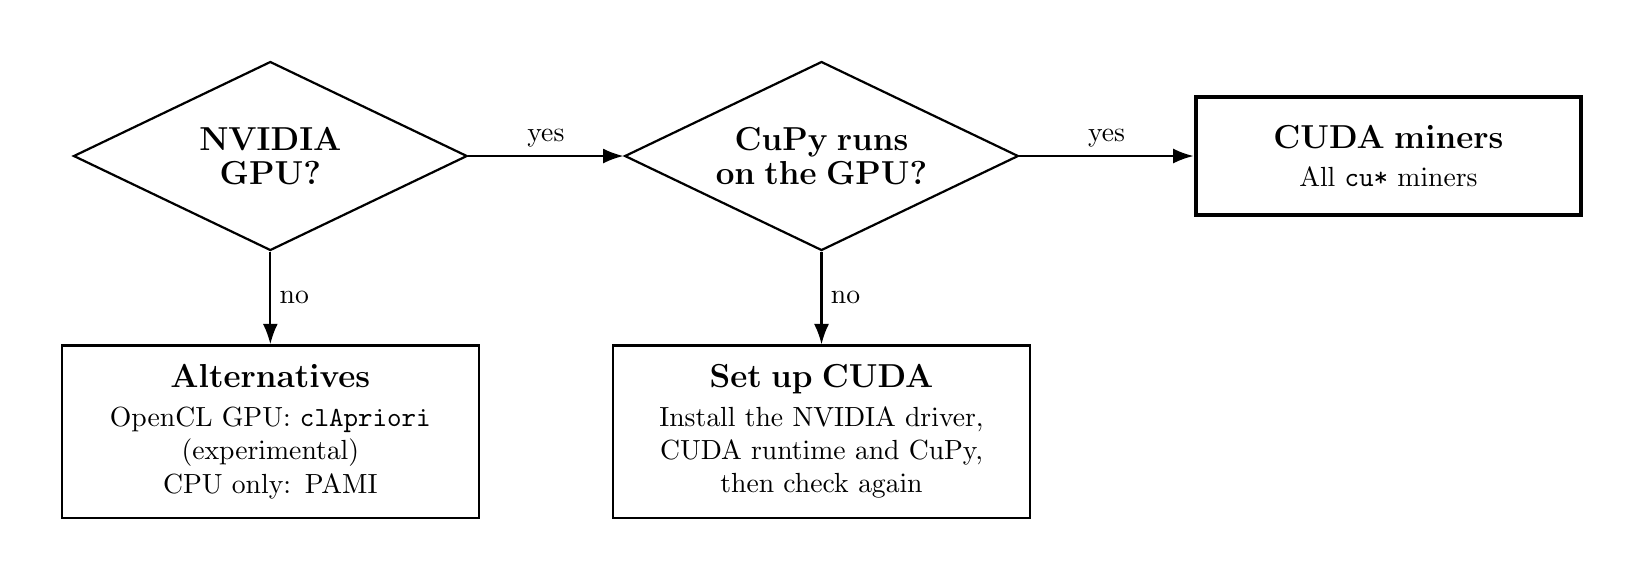
\begin{tikzpicture}[canvas]
\node[ask] (gpu) at (0,0) {\head{NVIDIA\\GPU?}};
\node[ask] (cuda) at (7,0) {\head{CuPy runs\\on the GPU?}};
\node[core,text width=4.4cm] (ready) at (14.2,0)
 {\head{CUDA miners}\\[2pt]\sub{All \texttt{cu*} miners}};
\node[box,text width=4.8cm] (other) at (0,-3.5)
 {\head{Alternatives}\\[2pt]\sub{OpenCL GPU: \texttt{clApriori}\\(experimental)\\CPU only: PAMI}};
\node[box,text width=4.8cm] (setup) at (7,-3.5)
 {\head{Set up CUDA}\\[2pt]\sub{Install the NVIDIA driver,\\CUDA runtime and CuPy,\\then check again}};
\draw[flow] (gpu.east) -- node[note,above] {yes} (cuda.west);
\draw[flow] (cuda.east) -- node[note,above] {yes} (ready.west);
\draw[flow] (gpu.south) -- node[note,right] {no} (other.north);
\draw[flow] (cuda.south) -- node[note,right] {no} (setup.north);
\end{tikzpicture}
\end{document}
